\begin{figure}
    \centering
    \begin{minipage}{0.45\textwidth}
        \centering
        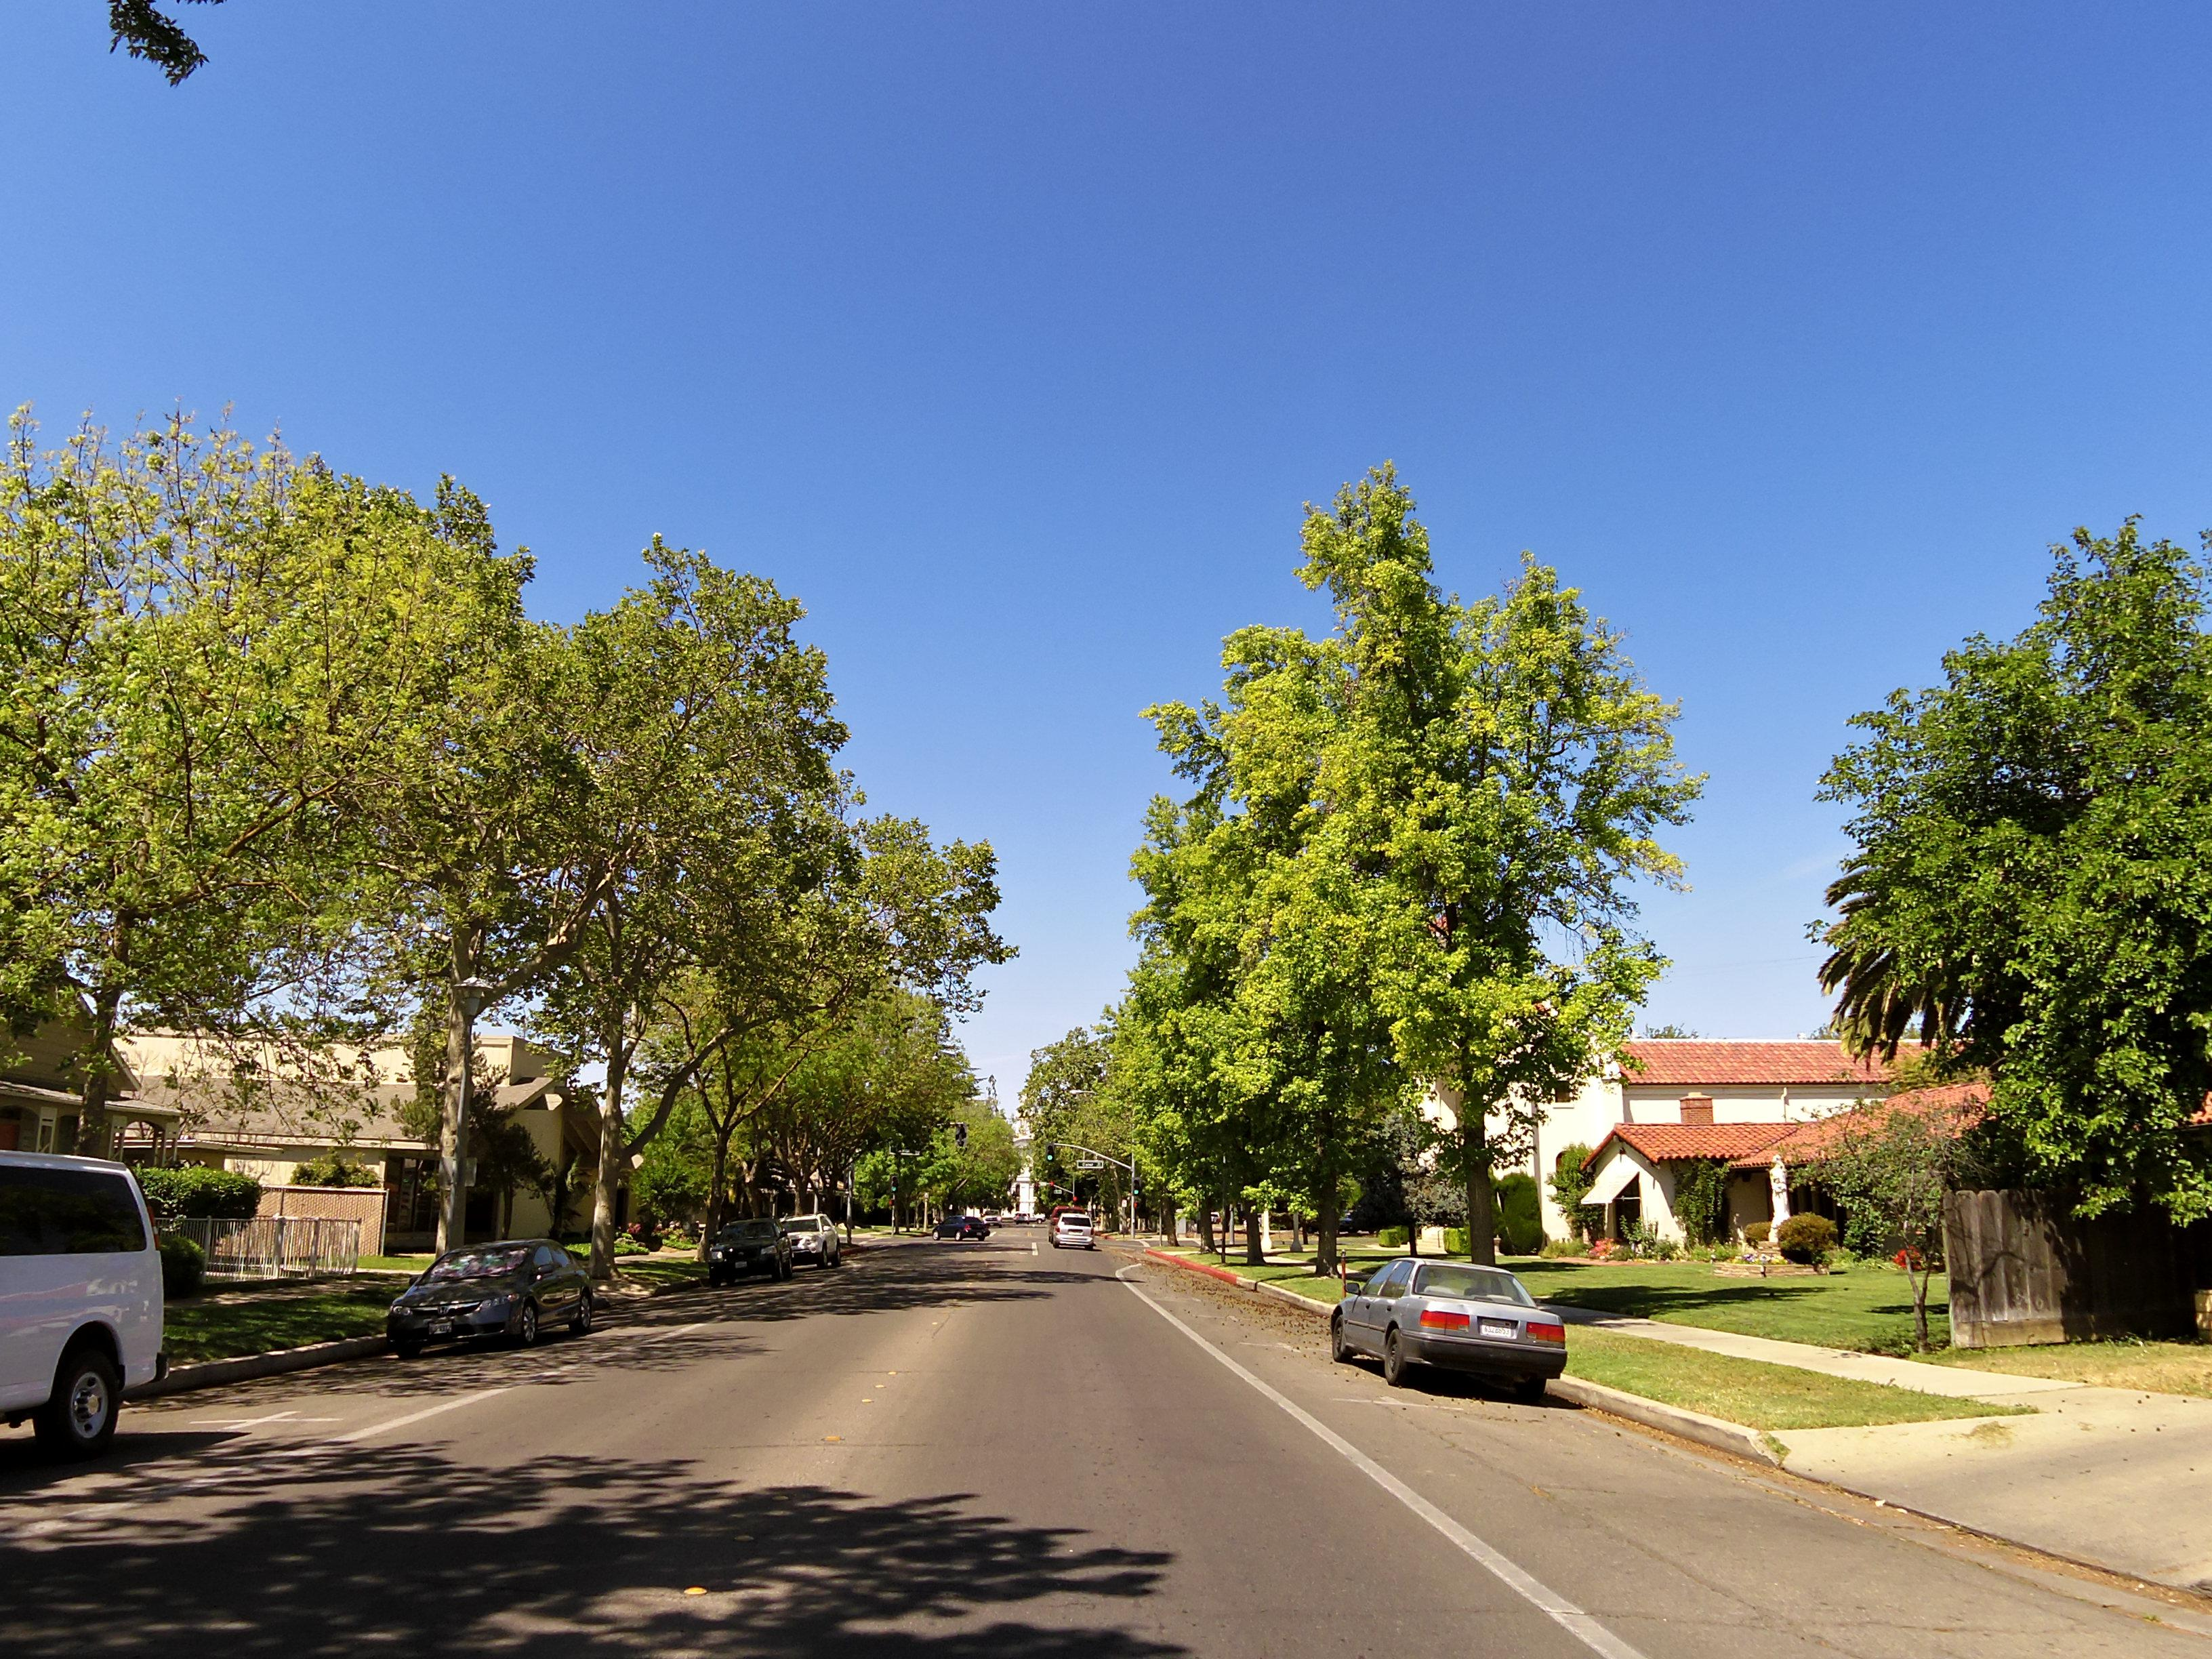
\includegraphics[width=0.9\textwidth]{figures/background/raw.jpg} % first figure itself
        \caption{An example street-level image as taken from a regular color camera.} \label{fig:background-raw}
    \end{minipage}\hfill
    \begin{minipage}{0.45\textwidth}
        \centering
        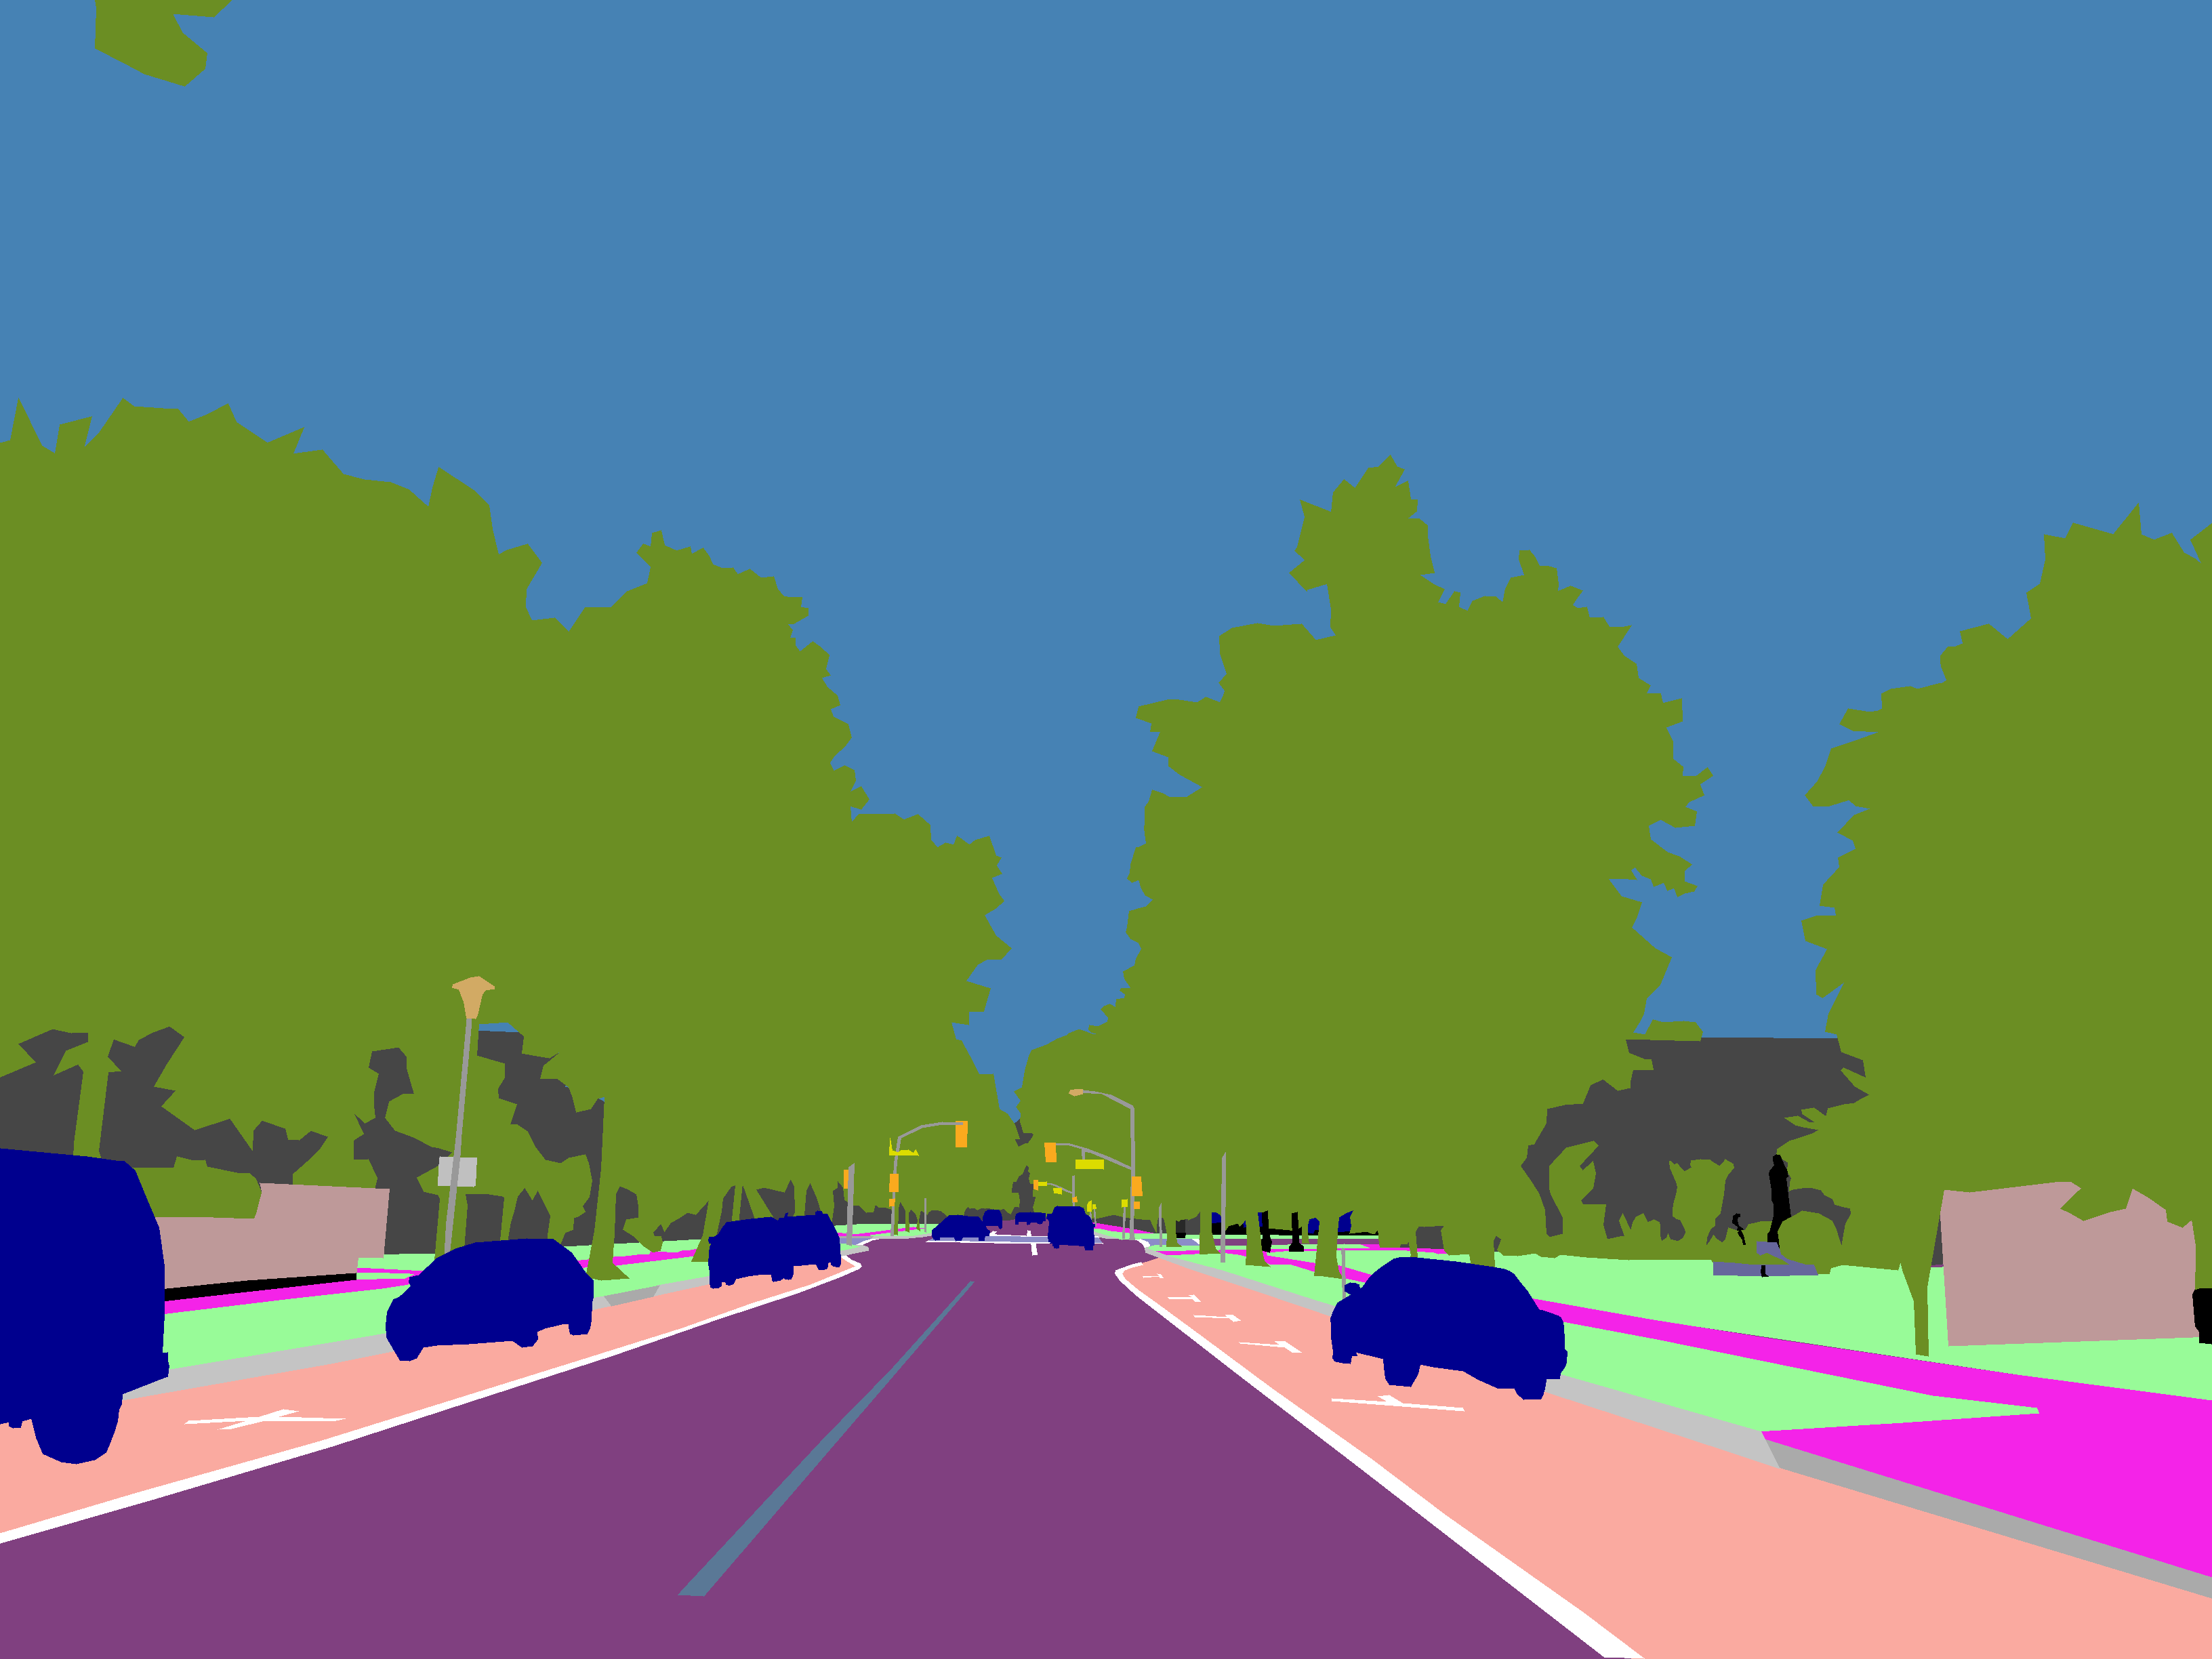
\includegraphics[width=0.9\textwidth]{figures/background/segmented.png} % second figure itself
        \caption{The segmented version of the image, each color representing a different class.} \label{fig:background-segmented}
    \end{minipage}
\end{figure}